\documentclass[]{article}

\usepackage{amsmath}
\usepackage{amsfonts}
\usepackage{amssymb}

\usepackage[]{algorithm2e}

\usepackage{booktabs}
\usepackage{rotating}

%%% for dags
\usepackage{tikz}
\usetikzlibrary{arrows}
\usetikzlibrary{fit,positioning, backgrounds}


%opening
\title{Consensus clustering for Bayesian mixture models: Supplementary materials}
\author{Stephen Coleman, Paul DW Kirk\, and Chris Wallace}

\begin{document}

\maketitle

\begin{abstract}

\end{abstract}

\section{Algorithms}

\begin{algorithm} \label{algorithm:simulationGeneration}
	%	\KwData{\(X=(x_1, \ldots, x_N)\)}
	\KwIn{
		%		A random seed $s$\\
		Distance between means \(\Delta_{\mu}\)\\
		A common standard deviation \(\sigma^2\)\\
		A number of clusters \(K\)\\
		The number of items to generate in total \(N\)\\
		The number of features to generate in total \(P\)\\
		An indicator vector of feature relevance \(\phi = (\phi_1, \ldots, \phi_P)\)\\
		The expected proportion of items in each cluster \(\pi=(\pi_1, \ldots, \pi_K)\)\\
		A method for sampling \(x\) times from the array \(y\), with weights \(\pi\): \emph{Sample}\((y, x, \pi)\)\\
		A method for permuting a vector \(x\): \emph{Permute}\((x)\)\\
		A method for generating a value from a univariate Gaussian distribution with mean \(\mu\) and standard deviation \(\sigma^2\): \emph{Gaussian}\((\mu, \sigma^2)\)\\
	}
	\KwOut{A dataset, $X$ \\ The generating cluster labels $c=(c_1, \ldots, c_N)$}
	%	\KwResult{how to write algorithm with \LaTeX2e }
	\Begin{
		%		\tcc{Set the random seed defining the sampling and permuting}
		%		$set.seed(s)$\;
		\tcc{initialise the empty data matrix}
		$X \leftarrow 0_{N \times P}$\;
		\tcc{create a matrix of \(K\) means}
		$\mu \leftarrow (\Delta_{\mu}, \ldots, K\Delta_{\mu})$\;
		\tcc{generate the allocation vector}
		\(c \leftarrow\) \emph{Sample}\((1:K, N, \pi)\)\;
		
		$\mathbf{M} \leftarrow \mathbf{0}_{N \times N}$\;
		\For{$p = 1$ \KwTo $P$}{
			\tcc{Test if the feature is relevant, if relevant generate data from a mixture of univariate Gaussians, otherwise draw all items from the same distribution}
			\If{$\phi_p = 1$}{
				
				%				\tcc{Permute the means associated with each cluster within the current feature to create independent features}
				$\nu \leftarrow$ \emph{Permute}$(\mu)$\;
				
				\For{$n = 1$ \KwTo $N$}{
					%					\tcc{Generate data defined by the original label}
					\(X(n, p) \leftarrow\) \emph{Gaussian}\((\nu_{c_n}, \sigma^2)\)
				}
			}
			\If{$\phi_p = 0$}{
				\For{$n = 1$ \KwTo $N$}{
					\(X(n, p) \leftarrow\) \emph{Gaussian}\((0, \sigma^2)\)
				}
			}
		}
		\tcc{Mean centre and scale the data}
		$X \leftarrow Normalise(X)$
	}
	\caption{Data generation for a mixture of Gaussian with independent features. This algorithm is implemented in the \texttt{generateSimulationDataset} function from the \texttt{mdiHelpR} package available at \texttt{www.github.com/stcolema/mdiHelpR}.}
\end{algorithm}

\section{The model}

\begin{figure}
	\centering
	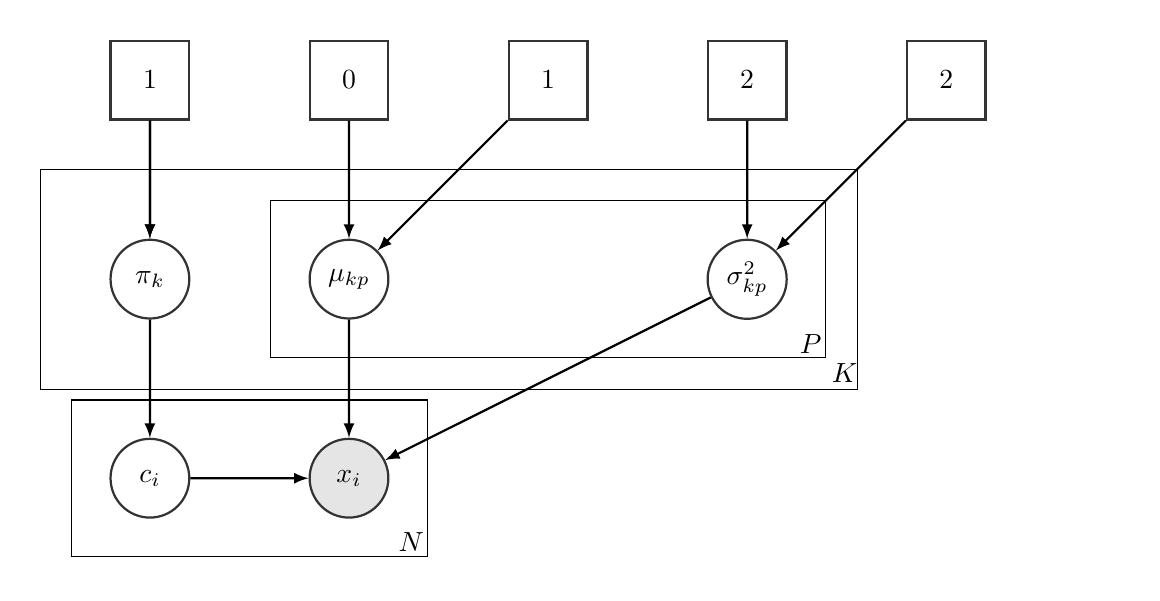
\begin{tikzpicture}[background rectangle/.style={fill=white!1}, show background rectangle, scale=.4, auto,>=latex']
		\tikzstyle{main}=[circle, minimum size = 10mm, thick, draw =black!80, node distance = 15mm]
		\tikzstyle{connect}=[-latex, thick]
		\tikzstyle{box}=[rectangle, draw=black!100]
		%\node[main] (k) {$K$ };
		\node[main, rectangle] (kappa) {$1$};
		\node[main, rectangle] (xi) [left =of kappa] {$0$ };
		\node[main, rectangle] (alpha) [left =of xi] {$1$ };
		%		\node[main] (k) [above =of alpha] {$K$};
		\node[main, rectangle] (alpha2) [right =of kappa] {$2$ };
		\node[main, rectangle] (beta) [right =of alpha2] {$2$ };
		\node[main] (pi) [below =of alpha] {$\pi_k$ };
		\node[main] (c_i) [below =of pi] {$c_i$};
		\node[main] (mu) [below=of xi] {$\mu_{kp}$};		
		\node[main] (sigma) [below =of alpha2] {$\sigma^2_{kp}$};
		\node[main, fill = black!10] (x_i) [below =of mu] {$x_i$};
		\node[rectangle, inner sep=-0.5mm, fit= (c_i) (x_i),label=below right:$N$, xshift=13mm, yshift=-1mm] {};
		\node[rectangle, inner sep=4.8mm,draw=black!100, fit= (c_i) (x_i)] {};
		\node[rectangle, inner sep=-0.8mm, fit= (mu) (pi) (sigma),label=below right:$K$, xshift=43mm, yshift=-5mm] {};
		\node[rectangle, inner sep=8.8mm, draw=black! 100, fit= (mu) (pi) (sigma)] {};
		\node[rectangle, inner sep=-0.5mm, fit= (mu) (sigma),label=below right:$P$, xshift=26mm, yshift=-1mm] {};
		\node[rectangle, inner sep=4.8mm, draw=black! 100, fit= (mu) (sigma)] {};
		\path 
		%		(k) edge [connect, bend right=30] (pi)
		%		(k) edge [connect, bend left=30] (c_i)
		%(k) edge [connect, bend left=30] (mu)
		%(k) edge [connect] (sigma)
		(alpha) edge [connect] (pi)
		(pi) edge [connect] (c_i)
		(alpha) edge [connect] (pi)
		(c_i) edge [connect] (x_i)
		(mu) edge [connect] (x_i)
		(sigma) edge [connect] (x_i)
		(xi) edge [connect] (mu)
		(kappa) edge [connect] (mu)
		(alpha2) edge [connect] (sigma)
		(beta) edge [connect] (sigma)
		%(k) edge[connect, bend right=30] (x_i)
		;
	\end{tikzpicture}
	\caption{Directed acyclic graph for the Bayesian mixture of Gaussians used.}
	\label{fig:simpleMixNormals}
\end{figure}


\begin{sidewaysfigure}
	\centering
	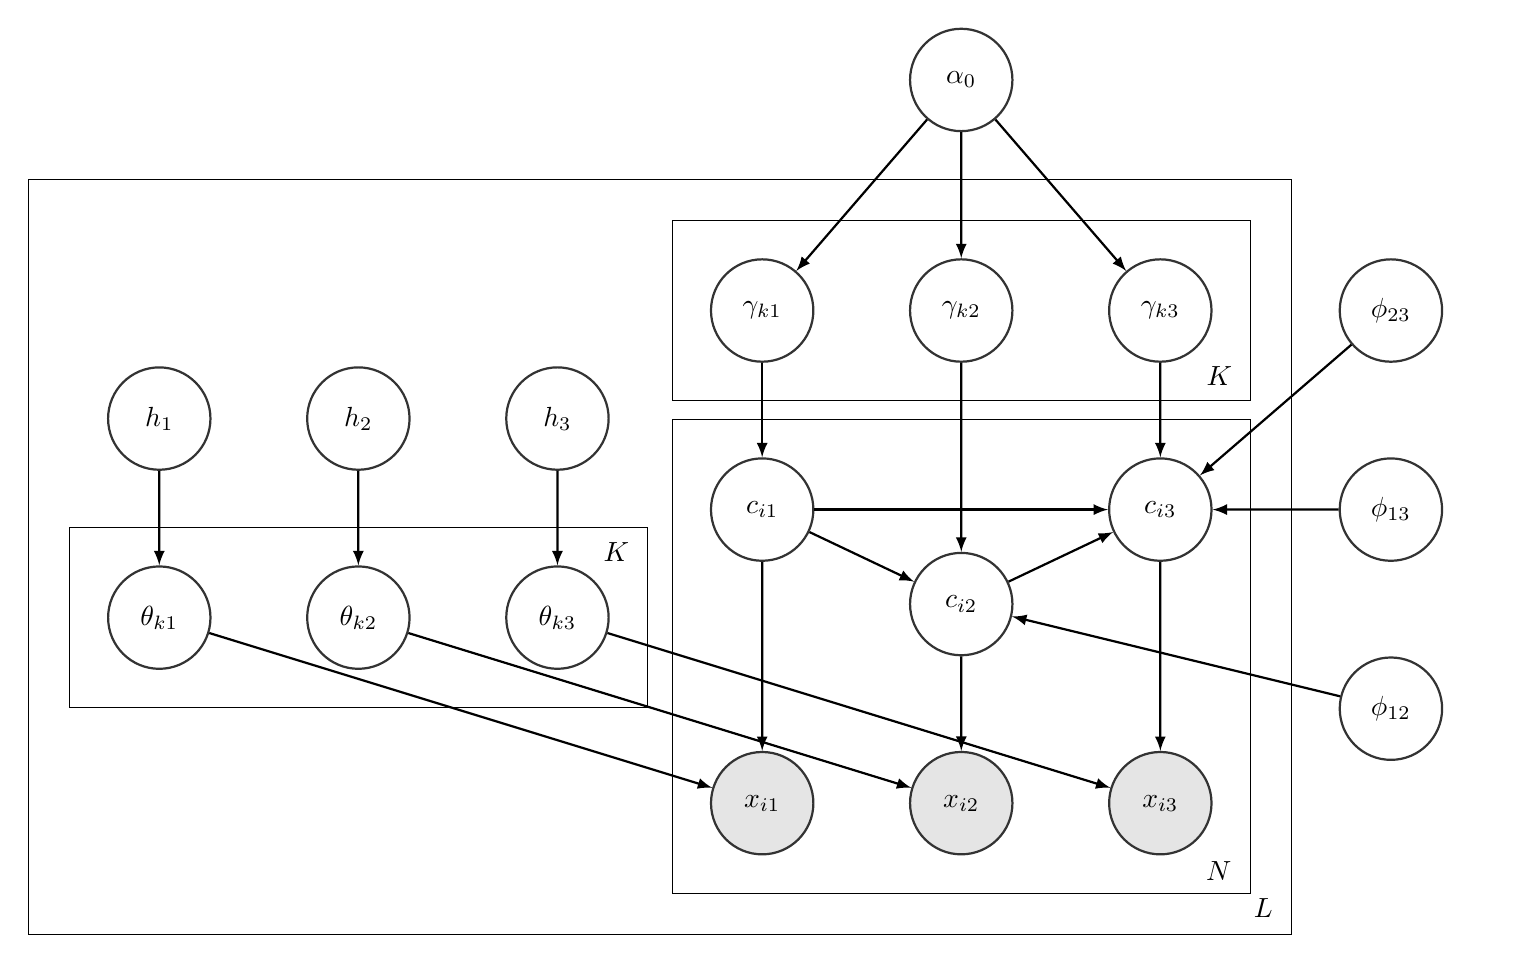
\begin{tikzpicture}[scale=.65, auto,>=latex']
	\tikzstyle{main}=[circle, minimum size = 13mm, thick, draw =black!80, node distance = 12mm]
	\tikzstyle{connect}=[-latex, thick]
	\tikzstyle{box}=[rectangle, draw=black!100]
	
	\node[main] (pi1) {$\gamma_{k1}$ };
	\node[main] (pi2) [right=of pi1] {$\gamma_{k2}$ };
	\node[main] (pi3) [right=of pi2] {$\gamma_{k3}$ };
	
	\node[main] (ci1) [below=of pi1] {$c_{i1}$};
	\node[main, node distance = 24mm] (ci2) [below=of pi2] {$c_{i2}$};
	\node[main] (ci3) [below=of pi3] {$c_{i3}$};
	
	\node[main, node distance = 16mm] (a) [above=of pi2] {$\alpha_0$ };
	
	\node[main, fill = black!10] (xi2) [below=of ci2] {$x_{i2}$}; 
	\node[main, fill = black!10] (xi1) [left=of xi2] {$x_{i1}$};
	\node[main, fill = black!10] (xi3) [right=of xi2] {$x_{i3}$};
	
	\node[main]  at (-4, -6) (theta3) {$\theta_{k3}$}; 
	\node[main] (theta2) [left=of theta3] {$\theta_{k2}$};
	\node[main] (theta1) [left=of theta2] {$\theta_{k1}$};
	
	
	\node[main] (h1) [above=of theta1] {$h_1$};
	\node[main] (h2) [above=of theta2] {$h_2$};
	\node[main] (h3) [above=of theta3] {$h_3$};
	
	\node[main, minimum size=1.3cm, node distance = 16mm] (phi13) [right=of ci3] {$\phi_{13}$}; 
	\node[main, minimum size=1.3cm] (phi12) [below=of phi13] {$\phi_{12}$};
	\node[main, minimum size=1.3cm] (phi23) [above=of phi13] {$\phi_{23}$};
	
	\node[rectangle, inner sep=-0.5mm, fit= (ci1) (ci2) (ci3) (xi1) (xi2) (xi3),label=below right:$N$, xshift=5mm, yshift=0mm] {};
	\node[rectangle, inner sep=4.8mm,draw=black!100, fit= (ci1) (ci2) (ci3) (xi1) (xi2) (xi3)] {};
	
	% \node[rectangle, inner sep=-0.8mm, fit= (theta1) (theta2) (theta3) (pi1) (pi2) (pi3) ,label=above right:$K$, xshift=63mm] {};
	% \node[rectangle, inner sep=4.8mm, draw=black! 100, fit= (theta1) (theta2) (theta3) (pi1) (pi2) (pi3)] {};
	
	\node[rectangle, inner sep=-0.8mm, fit= (theta1) (theta2) (theta3) ,label=above right:$K$, xshift=24mm] {};
	\node[rectangle, inner sep=4.8mm, draw=black! 100, fit= (theta1) (theta2) (theta3)] {};
	
	\node[rectangle, inner sep=-0.8mm, fit=  (pi1) (pi2) (pi3) ,label=below right:$K$, xshift=24mm] {};
	\node[rectangle, inner sep=4.8mm, draw=black! 100, fit= (pi1) (pi2) (pi3)] {};
	
	\node[rectangle, inner sep=-0.8mm, fit= (ci1) (ci2) (ci3) (xi1) (xi2) (xi3) (theta1) (theta2) (theta3) (pi1) (pi2) (pi3) (h1) (h2) (h3),label=below right:$L$, xshift=37mm, yshift=-5mm] {};
	\node[rectangle, inner sep=10.0mm, draw=black! 100, fit= (ci1) (ci2) (ci3) (xi1) (xi2) (xi3) (theta1) (theta2) (theta3) (pi1) (pi2) (pi3) (h1) (h2) (h3)] {};
	
	\path (pi1) edge [connect] (ci1)
	(pi2) edge [connect] (ci2)
	(pi3) edge [connect] (ci3)
	
	(ci1) edge [connect] (xi1)
	(ci2) edge [connect] (xi2)
	(ci3) edge [connect] (xi3)
	
	(ci1) edge [connect] (ci2)
	(ci1) edge [connect] (ci3)
	(ci2) edge [connect] (ci3)
	
	(theta1) edge [connect] (xi1)
	(theta2) edge [connect] (xi2)
	(theta3) edge [connect] (xi3)
	
	(h1) edge [connect] (theta1)
	(h2) edge [connect] (theta2)
	(h3) edge [connect] (theta3)
	
	(a) edge [connect] (pi1)
	(a) edge [connect] (pi2)
	(a) edge [connect] (pi3)
	
	(phi12) edge [connect] (ci2)
	(phi13) edge [connect] (ci3)
	(phi23) edge [connect] (ci3);
	
\end{tikzpicture}
	\caption{Directed acyclic graph for the Multiple Dataset Integration model for 3 datasets.}
	\label{fig:MDIDAG}
\end{sidewaysfigure}

\section{Additional results}
\subsection{Simulations}
\begin{sidewaysfigure} %[!tpb]
	\centering
	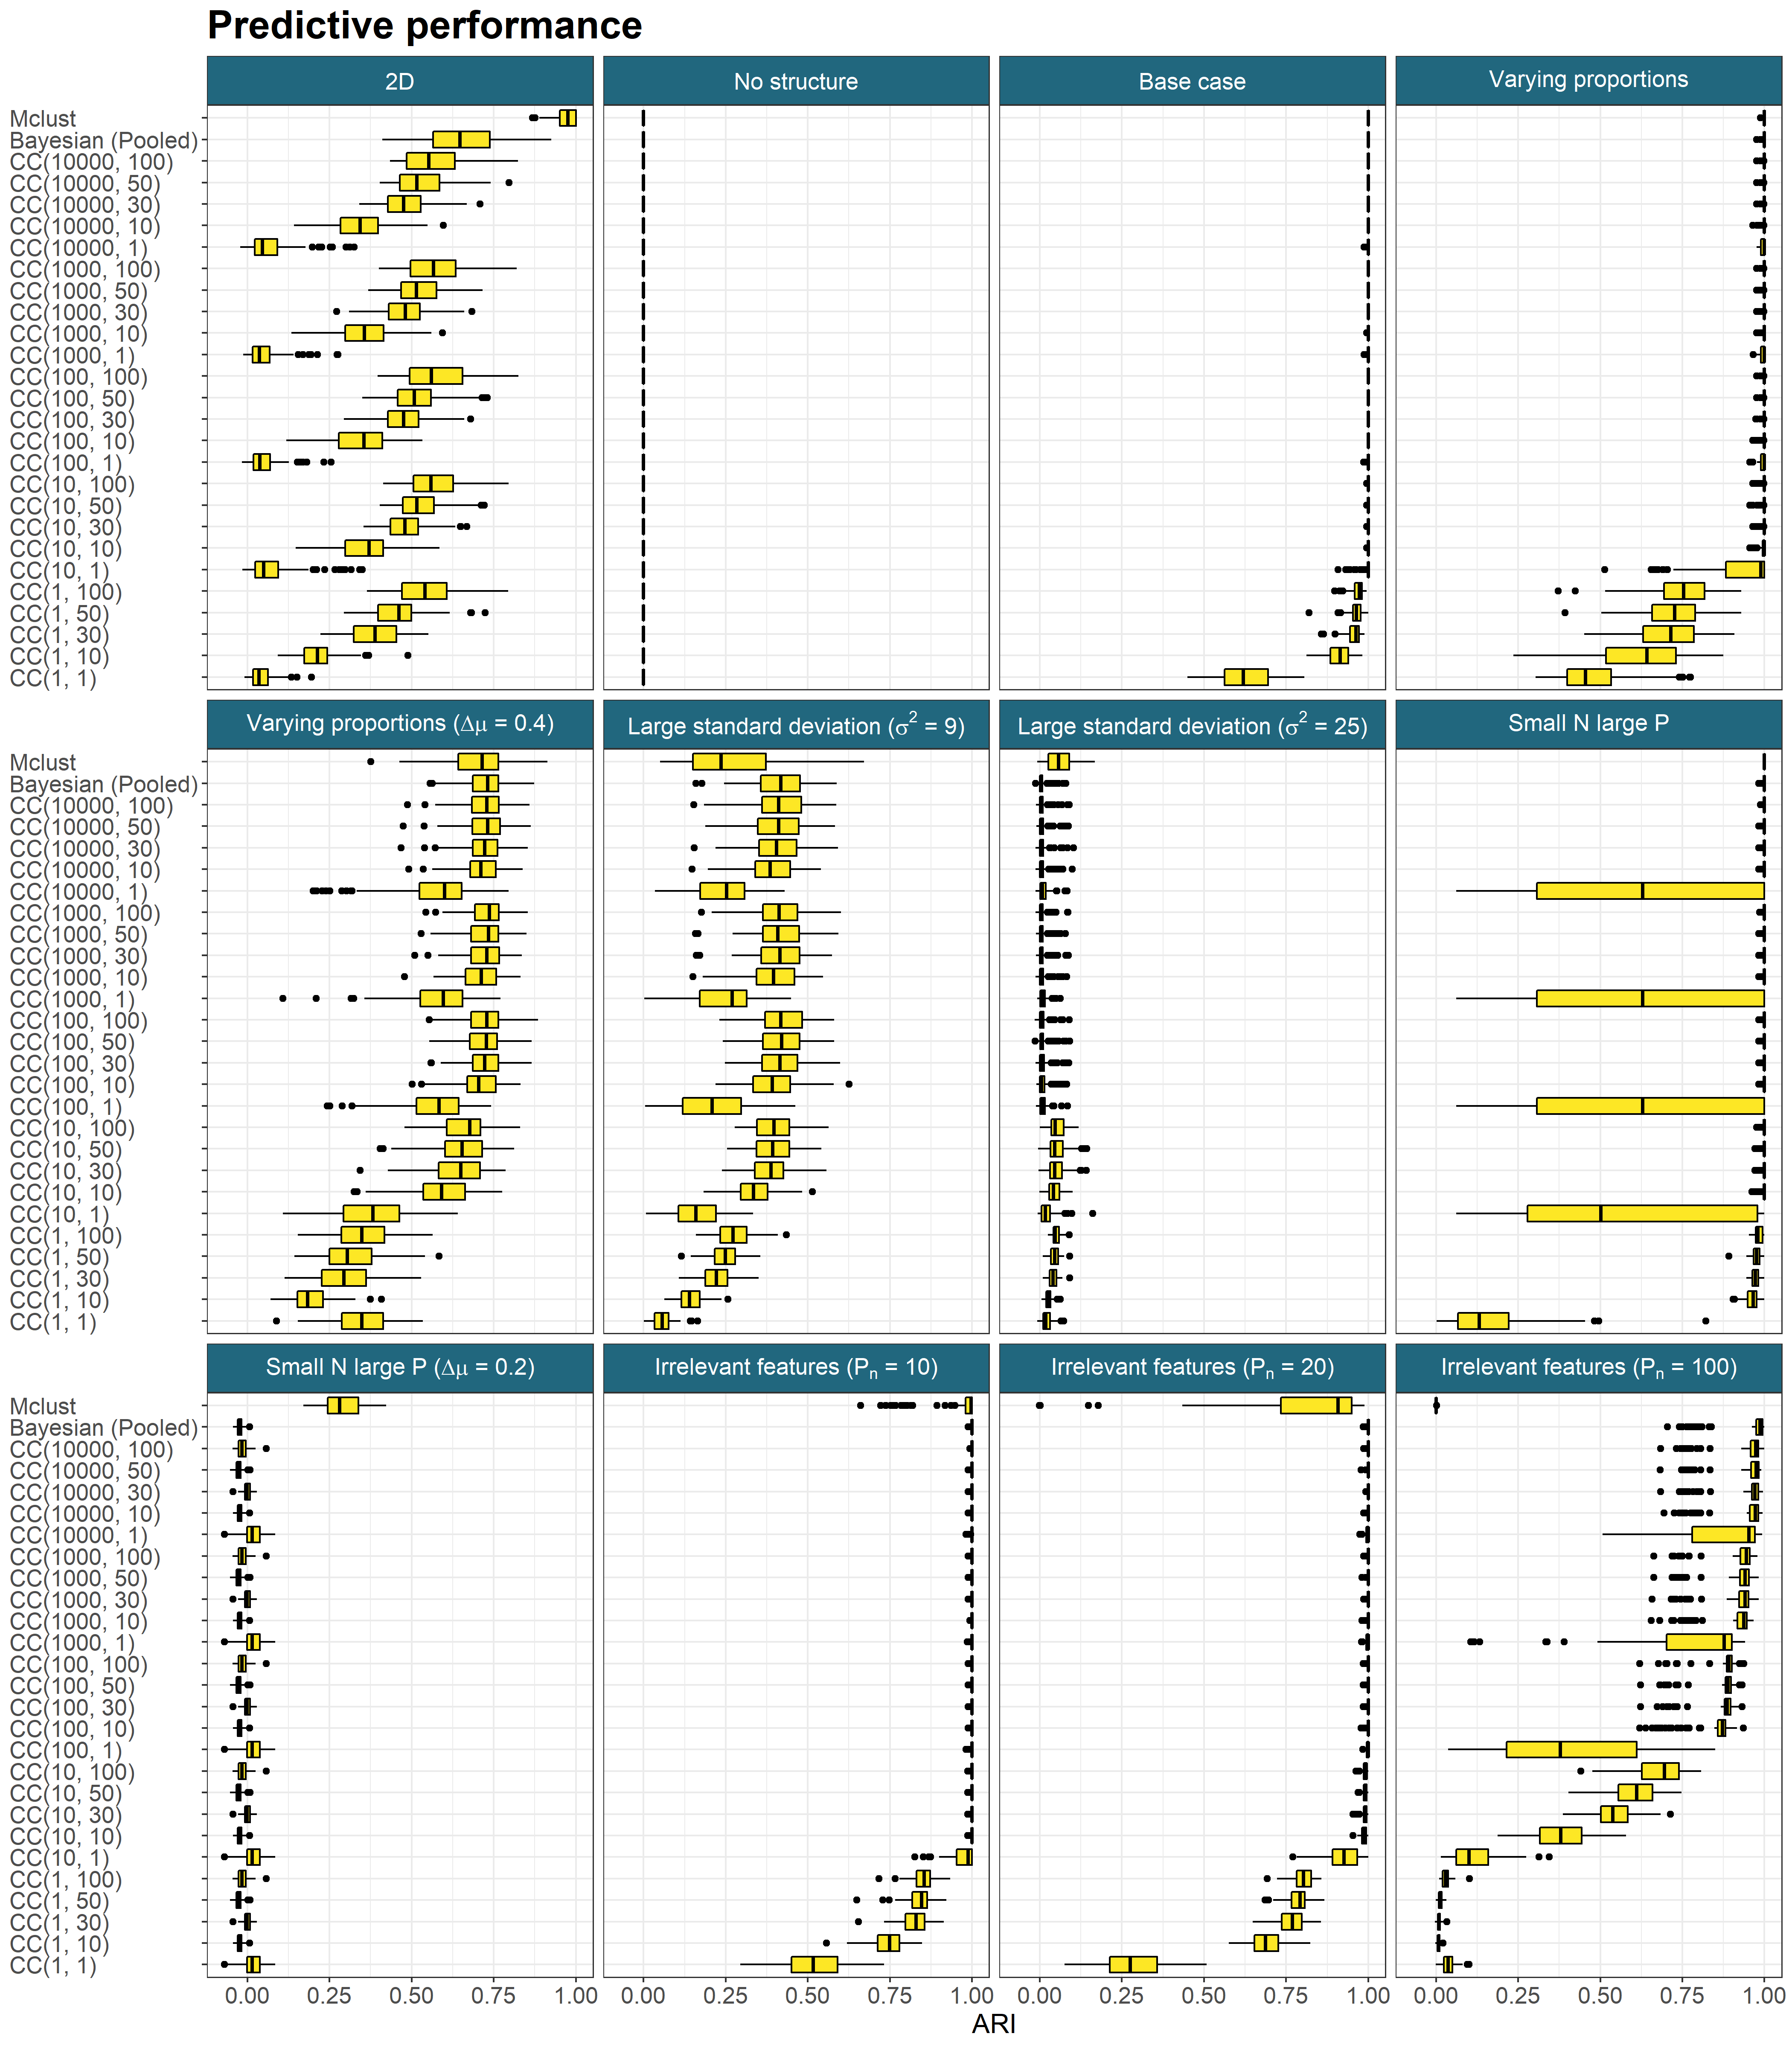
\includegraphics[scale=0.5]{./Images/Simulations/simulation_model_prediction.png}
	\caption{Predictive performance across all simulations. $CC(R, S)$ denotes consensus clustering using the $R^{th}$ sample from $S$ different chains.}
	\label{fig:simPrediction}
\end{sidewaysfigure}

\begin{sidewaysfigure} %[!tpb]
	\centering
	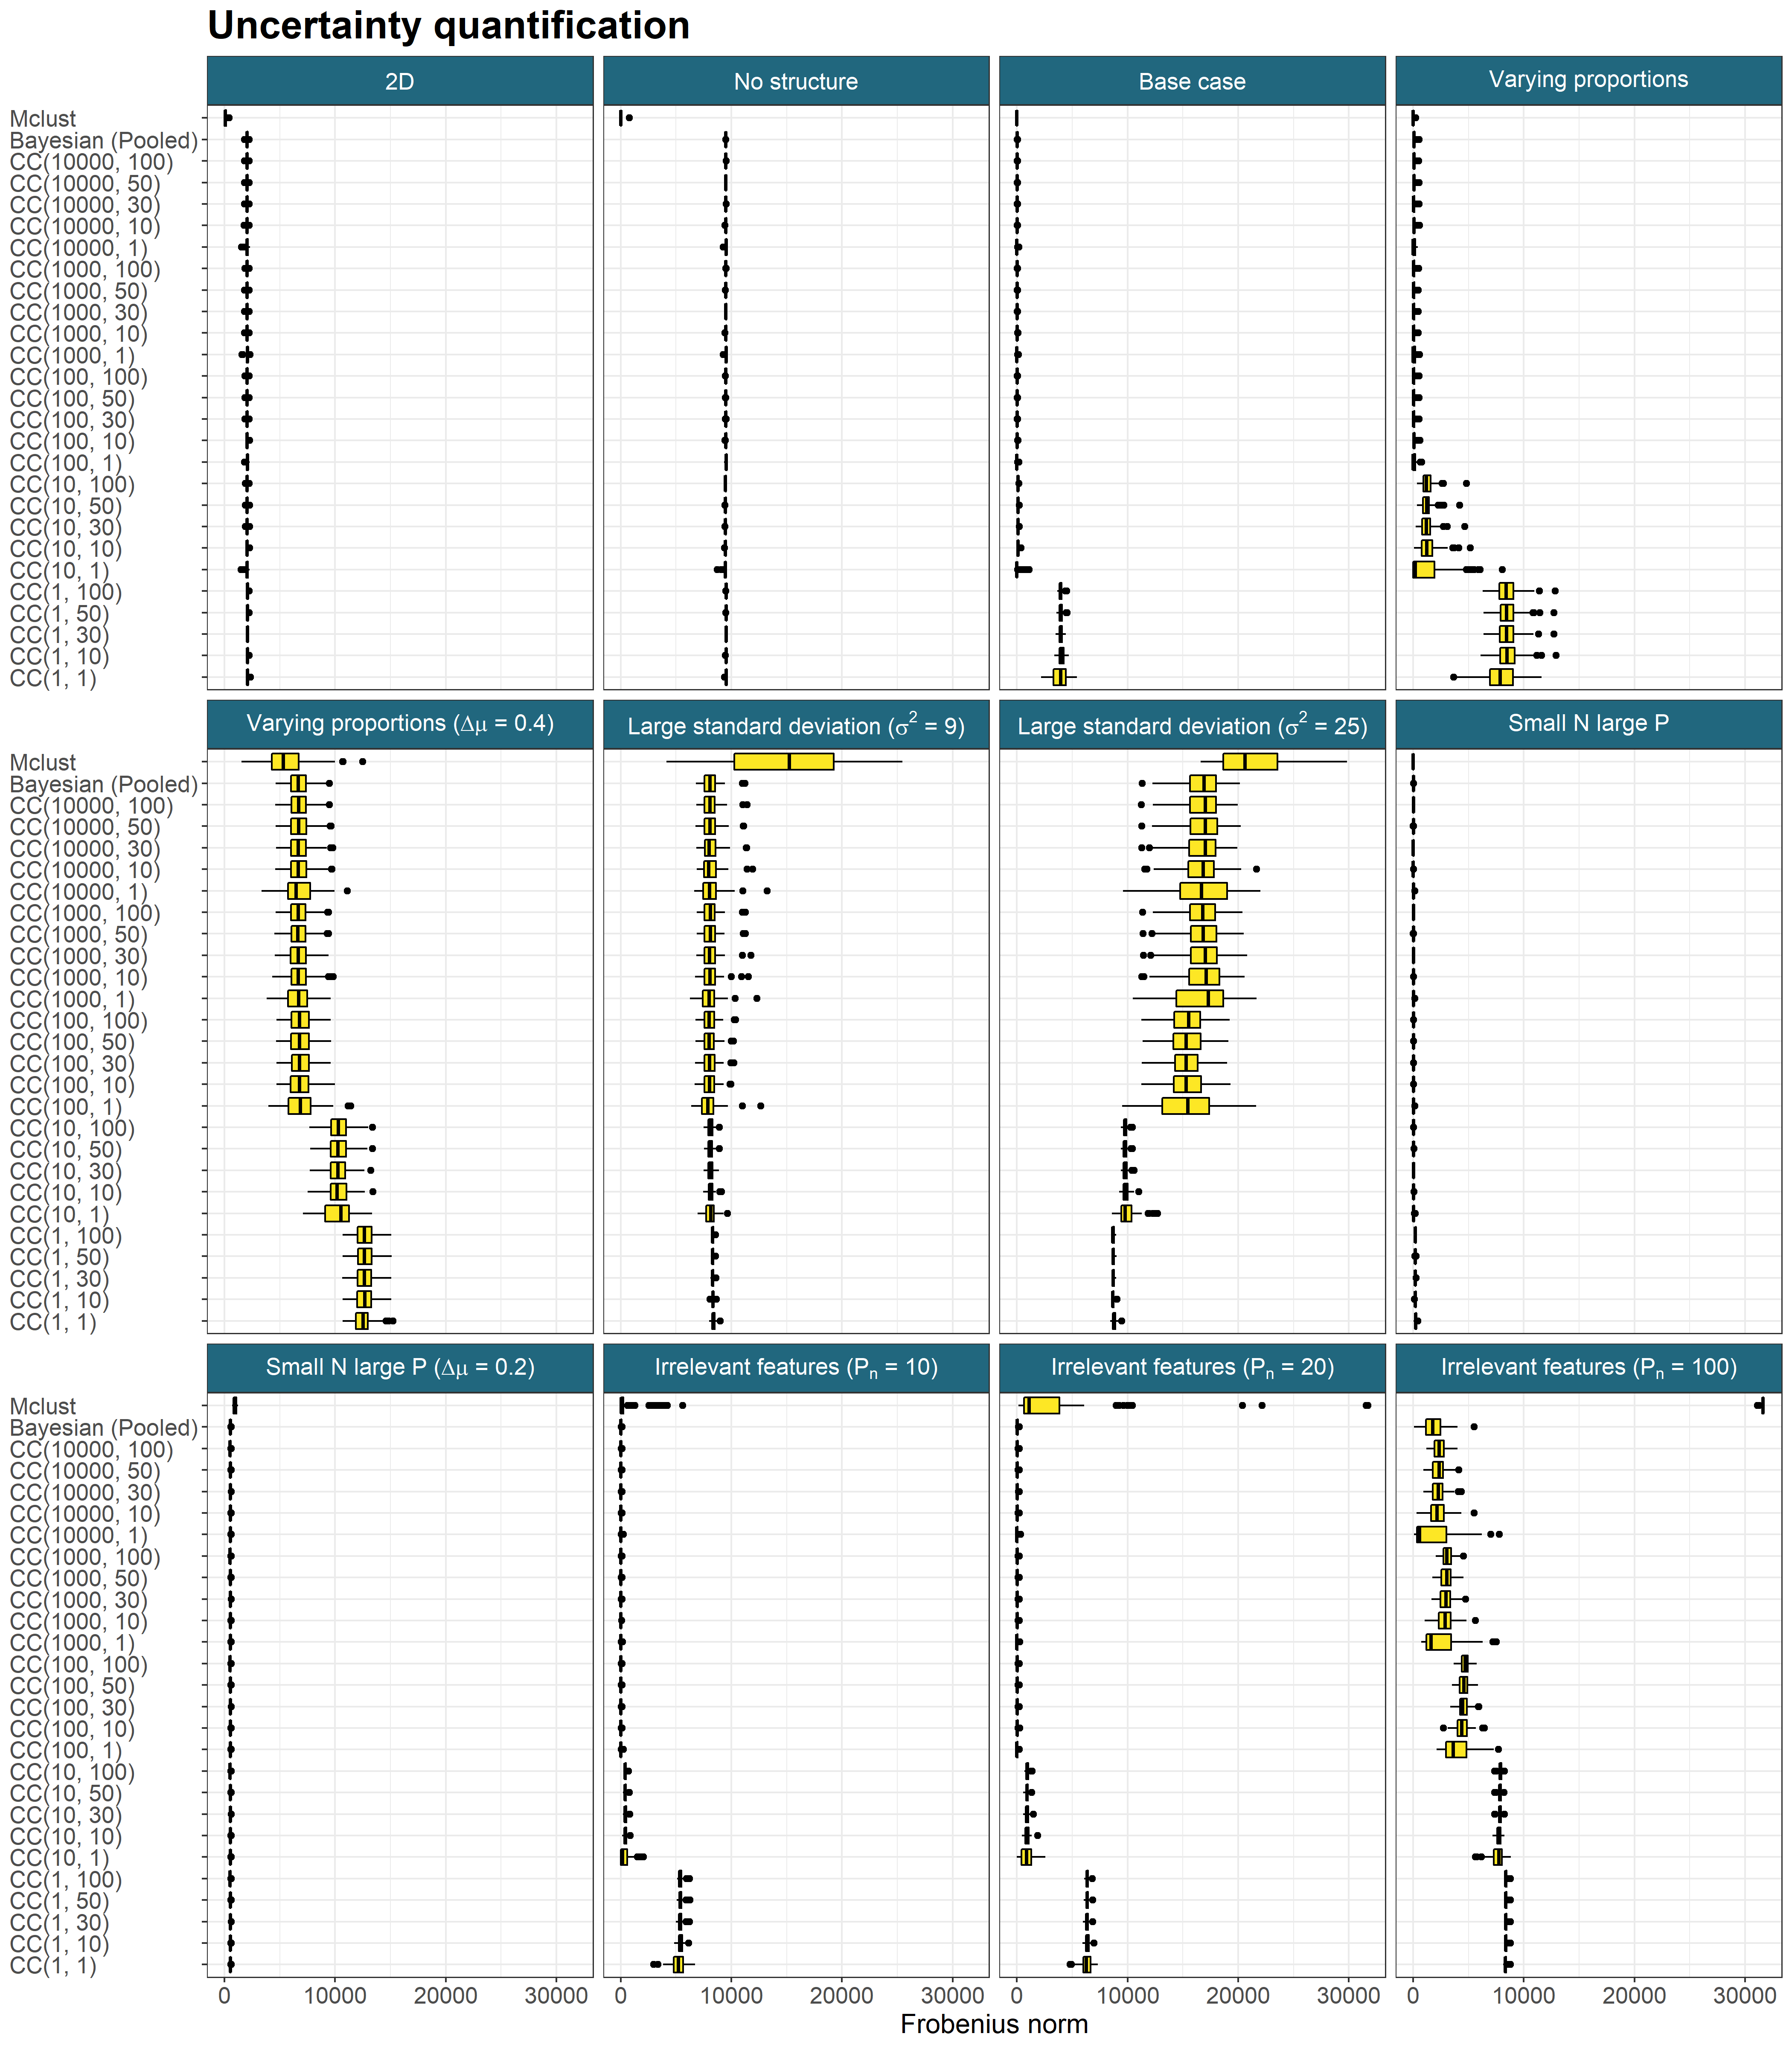
\includegraphics[scale=0.5]{./Images/Simulations/simulation_uncertainty.png}
	\caption{Frobenius norm across simulations. $CC(R, S)$ denotes consensus clustering using the $R^{th}$ sample from $S$ different chains. Lower values are better.}
	\label{fig:simUncertainty}
\end{sidewaysfigure}

\subsection{Yeast}

\begin{sidewaysfigure} %[!tpb]
	\centering
	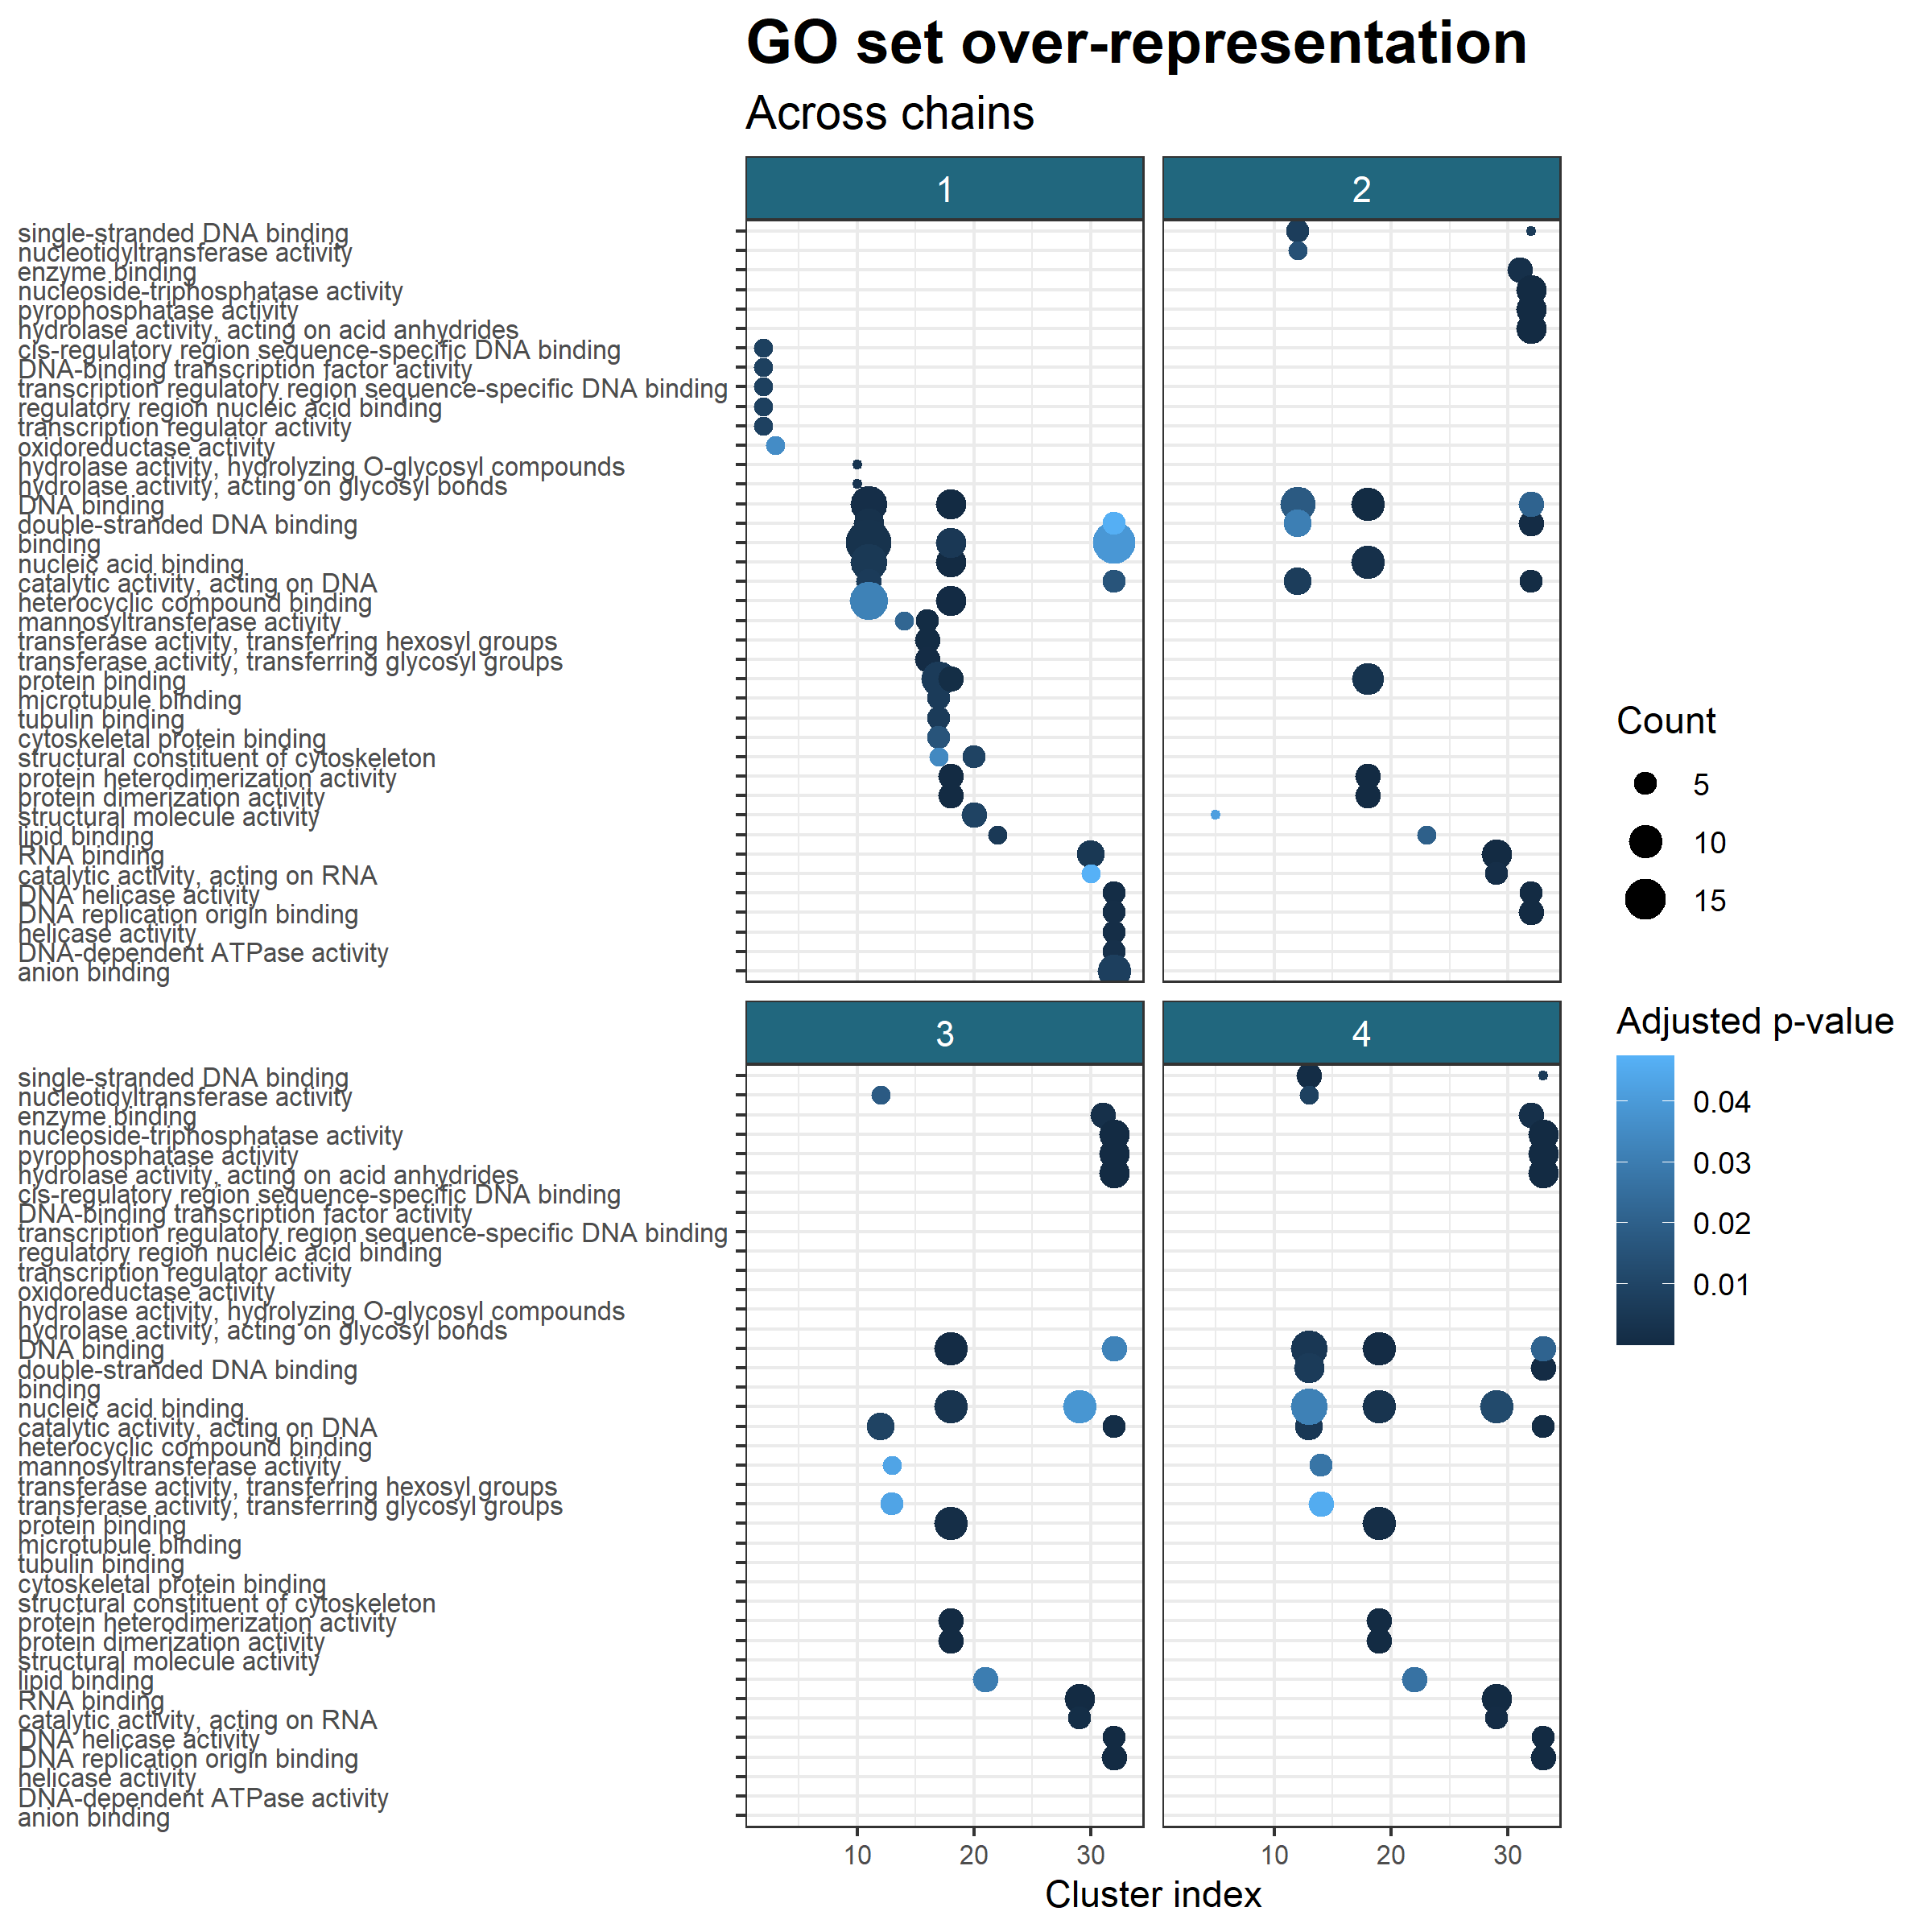
\includegraphics[scale=0.5]{./Images/Yeast/GOoverRepresentationBayesChains.png}
	\caption{The GO enrichment is very similar across chains.}
	\label{fig:yeastGOchains}
\end{sidewaysfigure}

\end{document}
